\documentclass{article}

\title{A swarm of replicated state machines}
\subtitle{A glance on the Internet Computer replicas through the lens of state machine replication.}
\date{2021-12-01}
\modified{2021-12-01}

\keyword{ic}

\begin{document}
\section*

In this article, we shall view the Internet Computer (IC) through the lens of distributed system design.
As most other blockchains, the IC achieves fault-tolerance using strategy called \href{https://en.wikipedia.org/wiki/State_machine_replication}{state machine replication}.
We shall take a close look at some design choices that make the IC fast, scalable, and secure.

\section{state-machine}{The state machine}

Before we dive into the internals of the protocol, let's first define the \href{https://en.wikipedia.org/wiki/Finite-state_machine}{state machine} that we'll be dealing with.
Nodes participating in the Internet Computer are grouped into units called \emph{subnet blockchains}, or simply \emph{subnets}.
Nodes in the same subnet run their own instance of the core Internet Computer Protocol (i.e., they form an independent peer-to-peer network and reach consensus independently from other subnets).
We'll model as a state machine the computation that nodes in the same subnet perform.

Let's play by the book and define components of our state machine:
\begin{description}
\term{Inputs}{
  The key product of the consensus protocol is a sequence of blocks containing messages for canisters hosted by the subnet.
  These blocks are the inputs of our state machine.
}
\term{Outputs}{
    In our model, the main artifact of the execution is a data structure called \emph{state tree}.
    We'll learn more about state trees in a moment.}
\term{States}{
  The single most important thing that the Internet Computer does is hosting canisters.
  Thus we'll define the state as a data structure containing everything we need to serve canisters installed on the subnet, including but not limited to:
  \begin{itemize}
  \item \href{https://webassembly.org/}{WebAssembly} modules and configuration of the canisters.
  \item Memory and stable memory of those canisters.
  \item Messages in canister mailboxes.
  \item Results of the recent ingress messages.
  \end{itemize}
}
\term{Transition function}{
  When a replica receives a block, it
  \begin{itemize}
  \item Injects messages from the block into the canister mailboxes.
  \item Picks some canisters for execution according to a deterministic scheduling algorithm.
  \item Executes the messages on the selected canisters and records the execution results.
  \end{itemize}
  All of the above modifies the data structure that we call ``state'' and acts as a transition function.
  Note that we can call this procedure a \emph{function} only if it's deterministic: given the same block and the same original state, the replica will modify the state in exactly the same way.
  Thanks to the careful design of execution algorithms and guarantees that WebAssembly provides, the procedure is indeed deterministic.
}
\term{Output function}{
  Once a replica processed a block, it computes a state tree.
  This tree can be used to inspect the results of the execution and validate the authenticity of those results.
  The deterministic procedure that constructs a state tree from the state is our output function.
}
\term{Initial state}{
  Each subnet starts its life with no canisters, no messages, and no results to inspect.
  It's as boring as it gets.
}
\end{description}

I call these state machines (one for each subnet) \emph{replicated} because each honest node on a subnet has an exact copy of the machine.

\subsection{checkpoints}{Checkpoints}

Let's say we want to add a new node to an existing subnet because a flood destroyed one of the data centers hosting the subnet.
This new node cannot start processing and proposing new blocks until it has the right state, the state that results from execution of all the blocks produced by this subnet so far.

One way to bring the node up to date is to download all those blocks and ``replay'' them.
This sounds simple, but if the rate of change is high and message execution is costly, the new node might need a \emph{lot} of time to catch up.
As the Red Queen put it: ``My dear, here we must run as fast as we can, just to stay in place.
And if you wish to go anywhere you must run twice as fast as that.''

Another solution is to create persistent snapshots of the state from time to time.
The peers can fetch and load those snapshots when they need help.
This method works really well for our state machine: it reduces the catch up time from days to minutes.
Let's call those persistent snapshots \emph{checkpoints}.

\begin{figure}[grayscale-diagram]
\marginnote{sm-components}{Components of the state machine: blocks as inputs, states, state trees as outputs, and checkpoints.}
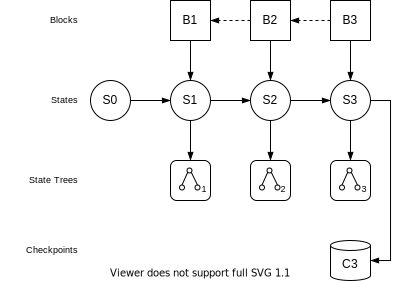
\includegraphics{/images/02-states.svg}
\end{figure}

\section{state-trees}{State trees}

The transition function is complex, but its details aren't very important for our discussion.
We can treat block processing as a black box.
Let's now see how we get the data out of the state machine.

There are quite a few bits of information that we want to access, for example:
\begin{itemize}
\item Replies to user requests.
\item Canister metadata, like module hashes or certified data entries.
\item Messages for other state machines (inter-subnet messages).
\end{itemize}

Furthermore, since we cannot trust any particular node, we want to have some authenticity guarantees for the data we get back.
Sounds easy: hash all the relevant bits of the state, collect a \href{https://en.wikipedia.org/wiki/Threshold_cryptosystem}{threshold signature} on that hash, and use the signature as a proof of state authenticity.
Problem solved?

But how do can we validate a single request status if we have a signature on the full state?
Collecting a separate signature for each request would solve the problem, but the cost of this approach is unacceptable from the performance point of view.

Wouldn't it be great to be able to ``zoom'' into different parts of the state to produce replies for different clients, while still having only a single hash to sign?
Enter state trees.

\begin{figure}[grayscale-diagram]
\marginnote{st-structure}{The logical structure of a state tree.}
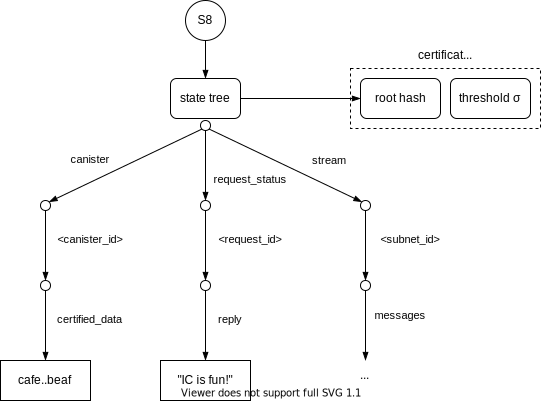
\includegraphics{/images/02-state-tree.svg}
\end{figure}

The state tree is a data structure that contains all outputs of our state machine in a form of a \href{https://en.wikipedia.org/wiki/Merkle_tree}{merkle tree}.
Once the gears of the execution stopped, the system computes the root hash of the state tree corresponding to the newly computed state, starts collecting a threshold signature for that hash, and moves on to the next block.

\subsection{tree-lookup}{Lookup}

Let's look at an example to see how the state tree does its magical zooming.
Assume that you sent a request with id \code{1355...48de} to the IC and you want to get back the reply.
As we now know, the system will put the reply into a state tree, so let's make a \href{https://smartcontracts.org/docs/interface-spec/index.html#http-read-state}{\code{read_state}} request with path \code{"/request_status/1355...48de/reply"}.

The replica processes our request in the following way
\begin{enumerate}
  \item Check that the caller has permission to look at the paths listed in the \code{read_state} request.
  \item Get the latest certified state tree (i.e. the state tree with a complete threshold signature on its root hash).
  \item Build the result tree that includes all the paths from the \code{read_state} request, with all the pruned branches replaced by their hashes.
  \item Combine the result tree with the threshold signature to form a full certified reply.
\end{enumerate}

The tree that you'll get back will look something like this:

\begin{figure}[grayscale-diagram]
\marginnote{responst-structure}{The logical structure of a tree containing a response to an ingress message.}
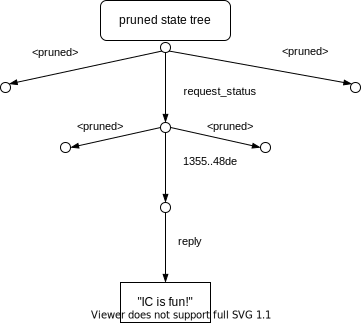
\includegraphics{/images/02-pruned-state-tree.svg}
\end{figure}

Even though the pruned tree is much smaller than the full state tree, both trees have exactly the same root hash.
So we can validate the authenticity of the pruned tree using the threshold signature that consensus collected for the root hash of the full state tree.

\section{state-transfer}{State transfer}

\subsection{state-artifact}{State as an artifact}

As we discussed in the \href{#checkpoints}{checkpoints} section, replicas periodically persist snapshots of its state to disk.
The main purpose of these snapshots is to speed up state recovery.
If a replica was out for a brief period of time, it can use its own checkpoint to recover more quickly than replaying all the blocks starting from the genesis.
Load the checkpoint, replay a few blocks, and you're ready to rock.
There is a more interesting case, however: a healthy replica can help other replicas catch up by sending them a recent checkpoint.

Replicas in a subnet communicate by exchanging \emph{artifacts} using a peer-to-peer protocol.
Most of these artifacts (e.g., user ingress messages, random beacons, state certifications) are relatively small, up to a few megabytes in size.
But the machinery for artifact transfer is quite general: the protocol supports fetching arbitrary large artifacts by slicing them into chunks, provided that there is a way to authenticate each chunk independently.
Furthermore, multiple chunks can be fetched in parallel from multiple peers.
Sounds a lot like \href{https://en.wikipedia.org/wiki/BitTorrent}{BitTorrent}, isn't it?

Before advertising a checkpoint, replica computes a \emph{manifest} for that checkpoint.
Manifest is an inventory of files constituting a checkpoint.
Files are sliced into chunks, and the manifest enumerates paths, sizes and cryptographic hashes of every file and every chunk of each file.
In our BitTorrent analogy, manifest plays a role of a \href{https://en.wikipedia.org/wiki/Torrent_file}{.torrent file}.
If we have a manifest, we know for sure how much data we need to fetch to construct a checkpoint, and how to arrange this data.
Hashes of file chunks in the manifest allow us to validate each chunk independently before we put it on disk.
Replicas use the hash of the manifest itself when they advertise a checkpoint in the peer-to-peer network.

\begin{figure}[grayscale-diagram]
\marginnote{checkpoint-advert}{A replica advertising a checkpoint as an artifact.}
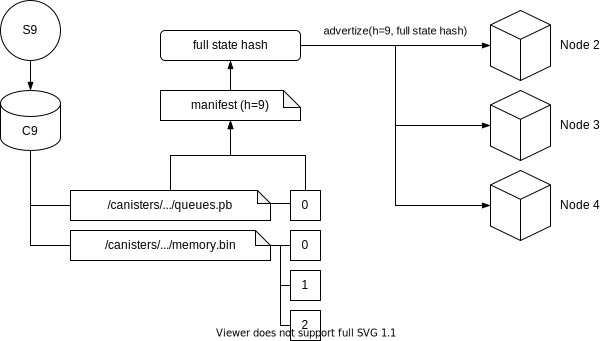
\includegraphics{images/02-checkpoint-artifact.svg}
\end{figure}

\subsection{trigger-transfer}{Triggering state transfer}

Let's assume that we have a replica that needs to fetch the latest checkpoint.
It listens to the peers, and discovers a few state artifacts with different hashes advertised by different peers.
How does our poor replica decide which state it needs to fetch?

As you might have guessed, the consensus subsystem armed with \href{https://en.wikipedia.org/wiki/Threshold_cryptosystem}{threshold signatures} comes to the rescue again.
Replicas gather a threshold signature on a full state hash and use that signature as a proof of checkpoint authenticity.
The result is an artifact containing a state height, a full state hash, and a threshold signature.
We'll call this artifact a \emph{catch-up package}.

The interaction between the replica consensus module and the state machine is something like the following
\begin{enumerate}
\item 
  Consensus sees a catch-up package for state 100 with a valid threshold signature and the state hash is \math{H\sub{100}}.
  Consensus asks the state machine "Hey, what's your state height?".
\item State machine: ``It's nine. Why?''
\item Consensus: ``We're missing out. Fetch the checkpoint for state 100, but only if it has root hash \math{H\sub{100}}.''
\item State machine: ``Sure, I'm on it.'' The state machine starts looking for state artifact advertisements with a matching hash.
\end{enumerate}

Yes, the consensus module can be a bit bossy sometimes, but it always acts with the best of intentions.

\subsection{incremental-sync}{Fetching states incrementally}

Let's now have a brief look at the most juicy part of state transfer, the actual state fetch protocol.
Let's suppose that we have a replica that has state 9 and it wants to catch up to state 100 with hash \math{H}.
\begin{enumerate}
\item The replica receives advertisements for checkpoint artifacts from other peers and picks the peers that advertize the state with the hash \math{H}.
\item The replica fetches the manifest of checkpoint 100 from one of the peers and validates that the manifest hash is indeed \math{H}.
\item The replica compares the manifest of checkpoint 9 that it has locally to the manifest of checkpoint 100.
\item 
  The replica copies all the chunks with the matching hashes from the old checkpoint into the new one.
  Why waste network bandwidth and fetch data you already have?
\item The replica fetches all the missing chunks from the peers, validates them against the manifest, and puts on disk them where they belong.
\end{enumerate}

When there are no more chunks to fetch, checkpoint 100 is complete, and the replica is ready to go.

\begin{figure}[grayscale-diagram]
\marginnote{checkpoint-construct}{A replica constructing a fresh checkpoint by re-using existing chunks and fetching the missing ones.}
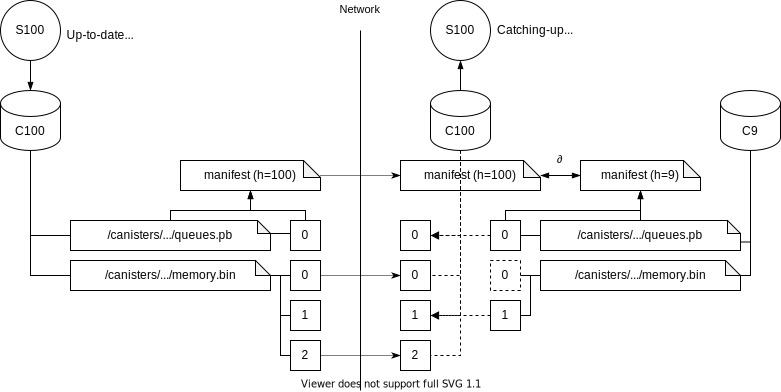
\includegraphics{/images/02-state-sync.svg}
\end{figure}

As you can see, the state transfer procedure is incremental: if the catching-up replica was offline for a brief period of time, it needs to fetch only the data that actually changed in the meantime.
Of course, a replica that has no checkpoints at all will have to fetch all the chunks to construct its first checkpoint.

\section{conclusion}{Conclusion}

In this article, we
\begin{itemize}
\item \href{#state-machine}{Abstracted} the complexity of block execution into a transition function of a finite state machine.
\item Marveled at how \href{#state-trees}{state trees} and \href{https://en.wikipedia.org/wiki/Threshold_cryptosystem}{threshold signatures} allow clients retrieve authentic replies by consulting only one replica.
\item Learned how replicas can their transfer states \href{#incremental-sync}{quickly} and \href{#trigger-transfer}{securely}.
\end{itemize}

This concludes our overview of how the IC implements state machine replication on the scale of a single subnet.
From that prospective, the IC as a whole is really a swarm of replicated state machines!

I made a few simplifications and omitted a lot of details to keep us focused on the replication aspect.
For example, we didn't look at how different subnets communicate with one another, how individual worker bees form the swarm.
This is a great topic that deserves an article of its own, so stay tuned!
\end{document}

